\chapter{Design Strategies}
We implemented a number of strategies for improving efficiency of raSAT: incremental search and refinement heuristics.
\section{Incremental search} \label{sec:incsearch}
{\bf raSAT} applies three incremental strategies, 
(1) {\em incremental windening}, (2) {\em incremental deepening} and (3) {\em incremental testing}. 
Let
$\varphi = \bigwedge \limits_{j=1}^m f_j > 0$ be the constraint to be solved.

\subsection{Incremental Windening and Deepening}
Given $0 < \gamma_0 < \gamma_1 < \cdots$ and $\varepsilon_0 > \varepsilon_1 > \cdots > 0$ raSAT's algorithm design with incremental widening and deepening is described in Algorithm~\ref{Al:incremental-widen-deepen}. The idea here is that raSAT starts searching within small interval and large value of threshold. If SAT is detected, the result can be safely returned. If the current intervals cannot satisfy the constraint (UNSAT is detected), larger intervals are consider. In the case of UNKNOWN, the threshold is not small enough to detect either SAT or UNSAT. As the result, raSAT decreases it and restarts the search. In Theorem~\ref{theorem:SAT-complete} and Theorem~\ref{theorem:UNSAT-complete}, the threshold $\gamma$ is not easy to calculate, but by incremental deepening, such threshold can be eventually reached because it does exist.
\begin{algorithm}
\begin{algorithmic}[1]
\State $i\gets 0$
\State $j\gets 0$
\While{true}
	\State $\Pi = \bigwedge\limits_{v_i \in V} v_i \in \langle -\gamma_i, \gamma_i \rangle$ 
	\If {$(\Pi, \varphi, \emptyset, \emptyset, \emptyset, \varepsilon_j, \bot) \to SAT$}
		\State \Return SAT
	\ElsIf {$(\Pi, \varphi, \emptyset, \emptyset, \emptyset, \varepsilon_j, \bot) \to UNSAT$}
		\If {$\gamma_i = +\infty$}
			\State \Return UNSAT
		\Else 
			\State $i \gets i + 1$
		\EndIf
	\Else 
		\State $j \gets j + 1$
	\EndIf
\EndWhile
\end{algorithmic}
\caption{Incremental Widening and Deepening}
\label{Al:incremental-widen-deepen}
\end{algorithm}
\begin{comment}
\begin{figure}[ht]
\begin{minipage}[b]{1.0\linewidth}
\centering
\begin{tabular}{c@{\qquad}c}
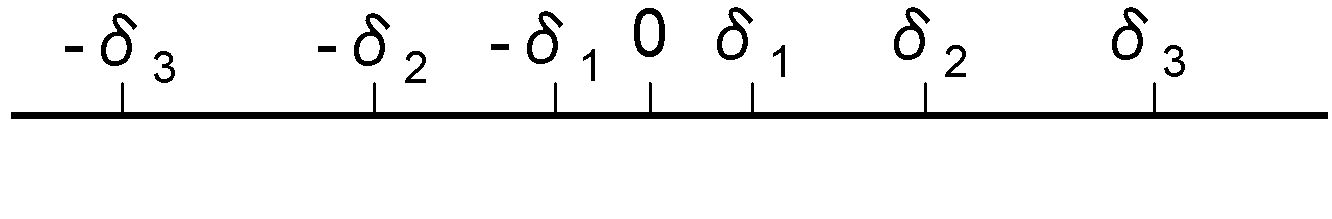
\includegraphics[height=0.4in,width=1.8in]{IncWiden.png} &
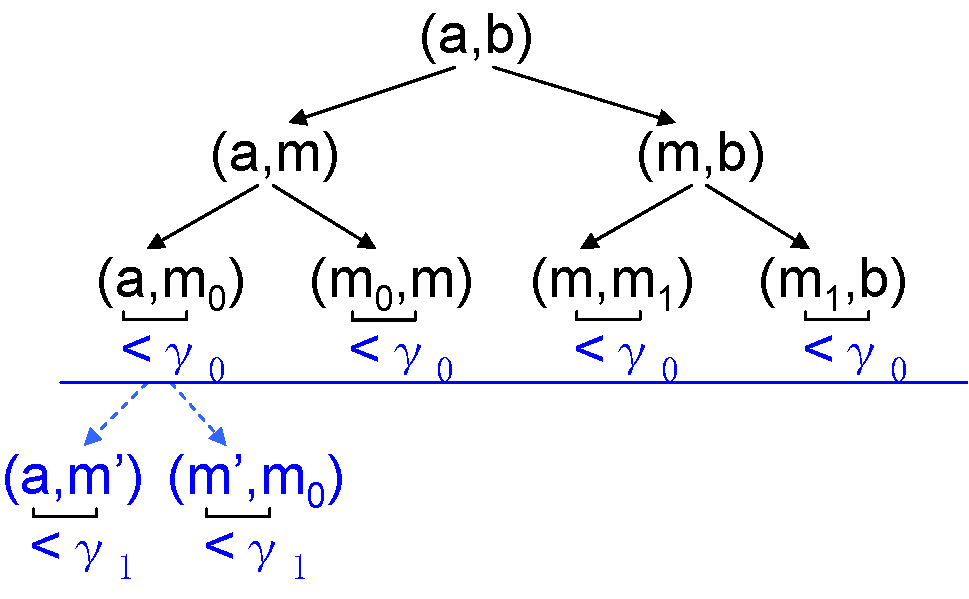
\includegraphics[height=1.2in,width=2in]{IncDeepen.png} \\
\mbox{(a) Incremenal widening} & \mbox{(b) Incremental Deepening} \\
\end{tabular}
\caption{Incremental Widening and Deepening}
\label{fig:incwid}
\end{minipage}
\end{figure

\begin{figure}[ht]
%\begin{minipage}[b]{1.0\linewidth}
\centering
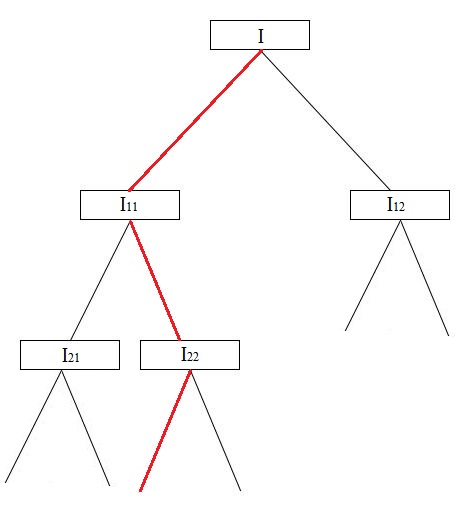
\includegraphics{depth-first-search.jpg} 
\caption{\textbf{raSAT} design} 
\label{fig:depth-first-search} 
%\end{minipage}
\end{figure} 
\end{comment}
\subsection{Incremental Testing}
One obstacle in testing is the exponentially large number of test instances (number of selected models). If $2$ values are generated for each of $n$ variables, $2^n$ test cases (combinations of generated values) will present. 
\begin{example}
Suppose $\{x, y\}$ is the set of variables which appears in the input constraint and let $\{2, 9\}$ and $\{5, 8\}$ are generated values for $x$ and $y$ respectively. In total $4$ test cases arise: $(x, y) = (2, 5), (2, 8), (9, 5), (9, 8)$.
\end{example}

In order to tackle the problem, the following strategies are proposed:
\begin{enumerate}
\item Restrict the number of test cases to $2^{10}$ by choosing most $10$ influential variables which are decided by the following procedures for generating multiple ($2$) test values.
\begin{itemize}
\item[$\bullet$] Select 10 inequalities by SAT-likelihood.
\item[$\bullet$] Select $1$ variable of each selected API using sensitivity.
\end{itemize}
\item Incrementally generate test values for variables to prune test cases that do not satisfy an inequality. This was proposed by \citeauthor{khanhReport} in \cite{khanhReport}:
\begin{itemize}
\item[$\bullet$] Dynamically sort the IA-SAT inequalities by SAT-likelihood such that the inequality which is less likely to be satisfiable will be prioritized.
\item[$\bullet$] Generate the test values for variables of selected inequalities.
\end{itemize}
\begin{example}
Let $x^2 > 4$ and $x*y > 0$ are two IA-VALID APIs to be tested and somehow they are sorted in that order, i.e. $x^2 > 4$ is selected before $x*y > 0$. Suppose $\{1, 3\}$ are generated as test values for $x$ which are is enough to test the first selected API, i.e. $x^2 > 4$. As a result of testing, $x = 1$ is excluded from the satisfiable test cases whilst $x = 3$ is not. Next, when $x*y > 0$ is considered, $y$ needs to be generated $2$ values, e.g. $\{-3, 4\}$ and two test cases $(x, y) = (3, -3), (3, 4)$ come out to be checked. In this example, $(x, y) = (1, -3)$ and  $(x, y) = (1, 4)$ are early pruned by only testing $x = 1$ against $x^2 > 4$ .
\end{example}
\begin{figure}[ht]
\centering
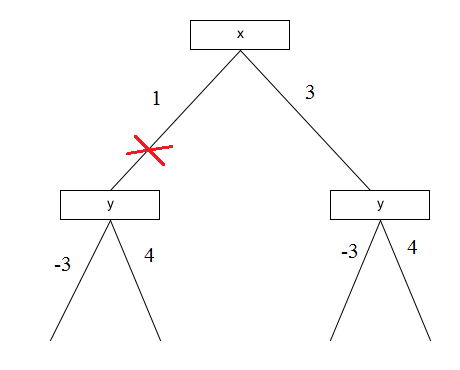
\includegraphics[scale=0.5]{incremental_test.png} 
\caption{Incremental Testing Example} 
\label{fig:incremental-test} 
%\end{minipage}
\end{figure} 
\end{enumerate}

\begin{definition}
Given an assignment from variables to intervals $\theta = \{v \mapsto i | v \in V\}$ in which $i \in \mathbb{I}$ and an inequality $f > 0$. Let $\langle l, h \rangle = f^{\theta^I}$, then the SAT-likelihood of $f > 0$ is $|\langle l, h \rangle \cap \langle l, h \rangle| / (h - l)$ which is denoted as $\varpi(f>0, \theta)$.
\end{definition}

\begin{definition}
Given an assignment from variables to intervals in the form of affine interval $\theta = \{v_i \mapsto a_{0i} + a_{1i}\epsilon_i | v_i \in V\}$ and a polynomial $f$. Let $a_0 + \sum\limits_{j = 1}^n a_j\epsilon_j = f^{\theta^I}$, then we define sensitivity of variable $v_i \in V$ by the value of $a_i$.
\end{definition}

\section{Refinement Heuristics} \label{sec:SATheuristics}
Suppose the number of variable is $nVar$ and initially the intervals assignment is represented by $\Pi = \bigwedge\limits_{v_i \in V} v_i \in \langle l_i, h_i \rangle$. If the interval of each variable is decomposed into two smaller ones, the new interval constraint becomes $\Pi' = \bigwedge\limits_{v_i \in V} (v_i \in \langle l_i, c_i \rangle \vee v_i \in \langle c_i, h_i \rangle)$ where $c_i$ is the decomposed point such that $l_i < c_i < h_i$. The number of boxes becomes $2^{nVar}$. The exponentially increase in the number of boxes affect the scalability of raSAT. To this point, raSAT applies two strategies for boosting SAT detection:
\begin{enumerate}
\item In \tiny{REFINE} \normalsize transition, the interval of one variable is selected for decomposition, raSAT chooses such variables through the following steps:
\begin{itemize}
\item[$\bullet$] Choose the inequality $f > 0$ in $\varphi^U$ with the least value of SAT-likelihood.
\item[$\bullet$] Within $f$, choose the variable $v_k$ with the largest value of sensitivity.
\end{itemize}
\item \sloppy After the interval of $v_k$ is decomposed, basically the box represented by ${\mathring{\Pi} = \bigwedge\limits_{v_i \in V} v_i \in \langle l_i, h_i \rangle}$ will become two boxes which are represented by ${\mathring{\Pi_1} = v_0 \in \langle l_0, h_0 \rangle \wedge \cdots \wedge v_k \in \langle l_k, c_k \rangle \wedge \cdots \wedge v_{nVar} \in \langle l_{nVar}, h_{nVar} \rangle}$ and ${\mathring{\Pi_2} = v_0 \in \langle l_0, h_0 \rangle \wedge \cdots \wedge v_k \in \langle c_k, h_k \rangle \wedge \cdots \wedge v_{nVar} \in \langle l_{nVar}, h_{nVar} \rangle}$. raSAT prepares the following strategies to choose one box to explore:
\begin{itemize}
\item[$\bullet$] the box with higher/smaller value of SAT-likelihood to explore in the next iteration, i.e. the result of SAT operation in \tiny $\Pi$\_SAT \normalsize is controlled so that the desired box will be selected, and
\item[$\bullet$] the box with higher/smaller inequalities that can be solved by IA and Testing.
\end{itemize}

\end{enumerate}
\begin{definition}
Given an assignment from intervals to variables ${\theta = \{v \mapsto i | v \in V\}}$ in which $i \in \mathbb{I}$ and a constraint $\bigwedge\limits_{i = 1}^nf_i > 0$. The SAT-likelihood of $\theta$ is defined as ${\min\limits_{i = 1}^n \varpi(f_i > 0, \theta)}$.
\end{definition}